\documentclass[12pt]{report}

\usepackage{graphicx}

\usepackage[francais]{babel}

\title{Mémoire de Fin d'étude}
\author{Abdellatif}

\begin{document}
\section*{Introduction général}
Les médicaments est toute substance ou composition présentée comme possédant des propriétés curatives ou préventives à l'égard des maladies humaines ou animales. Par extension, un médicament comprend toute substance ou composition pouvant être utilisée chez l'être humain ou l'animal ou pouvant leur être administrée, en vue d'établir un diagnostic médical ou de restaurer, corriger ou modifier leurs fonctions physiologiques en exerçant une action pharmacologique, immunologique ou métabolique \cite{ref} .\\
L'ensemble de la chaîne des médicaments (recherche, production, contrôle qualité, distribution en gros, délivrance aux patients, pharmacovigilance) est sous la responsabilité de spécialistes diplômés des médicaments, les pharmaciens \cite{ref2}.\\
La pharmacocinétique  a pour but d'étudier le devenir d'un médicament dans l'organisme. La détermination des paramètres pharmacocinétiques d'un médicament apporte les informations qui permettent de choisir les voies d'administration et d'adapter les posologies pour son utilisation future \cite{ref3}. \\ La bioinformatique est tout à la fois une science à l'interface entre l'informatique et la biologie , en vue de leur exploitation dans l'industrie des médicaments. a partir des systèmes informatiques intelligents pour résoudre les problèmes biologiques, dans notre cadre d'étude  qui représente la découverte des médicament .
Au cours de la dernière décennie, l'apprentissage en profondeur a connu un succès remarquable dans divers domaines de l'intelligence artificielle.
Développé à partir de la recherche précédente sur les réseaux de neurones artificiels,
cette technologie a une performance supérieure à celle d'autres algorithmes d'apprentissage automatique dans des domaines tels que l'image et la voix reconnaissance, traitement du langage naturel. La première vague d'applications d'apprentissage en profondeur dans la recherche pharmaceutique a émergé ces dernières années \cite{ref4} . \\
Nous avons partagé notre étude en cinq chapitres, et voici un guide pour aborder ce document :\\
\begin{enumerate}
\item La première chapitre présente le contexte de notre étude : la biochimie.
\item Le deuxième chapitre est consacré à la description, machine Learning et deep Learning et les principales déférences entre les deux techniques.
\item Le troisième chapitre consacré la bioinformatique qui  va lié les notions entre le problème biochimie  qui va être  résoudre par les technologies informatiques . 
\item Le quatrième chapitre contient la contribution qui va présente tous les environnements matériels et logiciels pour réaliser ce travail .
\item le cinquième chapitre contient résultat et discussion on va voir une comparaison entre notre solution et résultat avec les solutions qui existe .   

\end{enumerate}





\part{}
\documentclass[12pt]{report}
\usepackage{graphicx}
\usepackage{color}


\begin{document}



\chapter{Biochimie}

\includegraphics[width=350]{biochimie_head_fr.jpg} 
\newpage
\section{Introduction}
La biochimie implique l'étude des processus chimiques qui se produisent dans les organismes vivants dans le but ultime de comprendre la nature de la vie en termes moléculaires \cite{ref5} . Les études biochimiques reposent sur la disponibilité de techniques analytiques appropriées et sur l'application de ces techniques à l'avancement des connaissances sur la nature, et les relations entre les molécules biologiques, en particulier les protéines et les acides nucléiques, et la fonction cellulaire \cite{ref5} . Ces dernières années d'importants progrès ont été réalisés dans notre compréhension de la structure et de l'expression des gènes et dans l'application de techniques telles que la spectrométrie de masse à l'étude de la structure et de la fonction des protéines.
Le projet du génome humain en particulier a été à l'origine de développements majeurs dans la compréhension de nombreuses maladies humaines, en particulier le cancer, et dans l'identification de stratégies pouvant être utilisées pour lutter contre ces maladies \cite{ref5} .\\aujourd'hui les grandes recherches scientifiques engagés dans la recherche biochimique et biotechnologie L'objectif principal  est de comprendre comment les biomolécules et leurs interactions génèrent les structures et les processus biologiques observés dans les cellules, pour la compréhension des organismes en général.
\newpage
\section{Biochimie}
\subsection{Définition}
La \textbf{biochimie} est le domaine où se rencontrent chimie et biologie, La biochimie étudie donc particulièrement la corrélation entre la structure des molécules naturelles et les conséquences sur leur activité \cite{ref6} .\\
La biochimie permet de comprendre selon quels "processus chimiques" fonctionnent les organismes vivants, des plus simples comme les bactéries et les virus, jusqu'aux plus complexes, comme les insectes, les mammifères et surtout les humains  \cite{ref6}  .
\subsection{Biologie}
\subsubsection{Définition}
La \textbf{biologie} est la science du vivant. Elle recouvre une partie des sciences de la nature et de l'histoire naturelle des êtres vivants  \cite{ref6} .\\
\begin{figure}[h]
\begin{center}
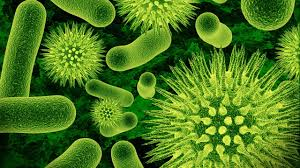
\includegraphics[width=300]{bio.jpg}
\caption{science du vivant}
\end{center}

\end{figure}


\subsection{La Chimie}
\subsubsection{Définition}
La \textbf{chimie} est une science de la nature qui étudie la matière et ses transformations,  et plus précisément les processus qui changent ou modifient l'identité de ces particules ou molécules de matière, dénommés réaction chimique, transformation, interaction, etc  \cite{ref6} .

\subsection{Les domaines de la biochimie}
la biochimie généralement est utilisé dans nombreuses domaines autour de l'organismes vivants telle que:
\begin{enumerate}
\item \textbf{pharmacologie} 
\item médecine
\item toxicochimie
\item génie génétique
\item structure des molécules
\end{enumerate}
Par exemple, la connaissance des mécanismes d'action d'une molécule sur un organisme permet l'élucidation de sa toxicité. Ce champ de recherche est celui de la toxicochimie  \cite{ref6} .

\section{pharmacologie}


\subsection{Définition}
La \textbf{pharmacologie} est la science de synthèse, emprunte des méthodes à l'ensemble des disciplines biologiques et physico-chimiques. Elle apporte les bases nécessaires à l'étude des mécanismes d'action des médicaments et des mécanismes de régulation des fonctions de l'organisme \cite{ref7}.
\subsection{pharmaceutique}
La biologie est l'un des sciences plus large et plus couteuse aux domaines des recherches scientifiques et parmi ces domaines la recherche pharmaceutique qui basent sur la production des médicaments et de trouvées nouveaux molécules. Le coute de la recherche augment car les molécules les plus faciles à trouvées ont déjà été utilisées, plus d'un milliard d'euros par médicament et le criblage en france. Les laboratoires doivent désormais s'intéresser à des molécules plus grosses, plus complexes \cite{ref7} .

\subsection{L'objectif de pharmaceutique}
les \textbf{médicaments} occupe une place importante dans l’exercice de la médecine \cite{ref7}.\\
La pharmacologie, qui se définit comme la science du médicament, contribue de manière incontournable à la compréhension des effets thérapeutiques attendus ou des effets indésirables observés lors de la prescription du médicament.\\On distingue :
\begin{enumerate}
\item Comprendre les bases pharmacologiques 
\item  la production des médicaments et de trouvées un nouveaux médicament

\end{enumerate}

\subsection{Qu'est ce qu'un médicament}
Il s'agit  de tout produit pouvant être administré à l'homme ou l'animal en vue  diagnostic médical  de restaurer, corriger ou modifier leur fonctions organiques \cite{ref7} . 
\begin{figure}[h]
\begin{center}
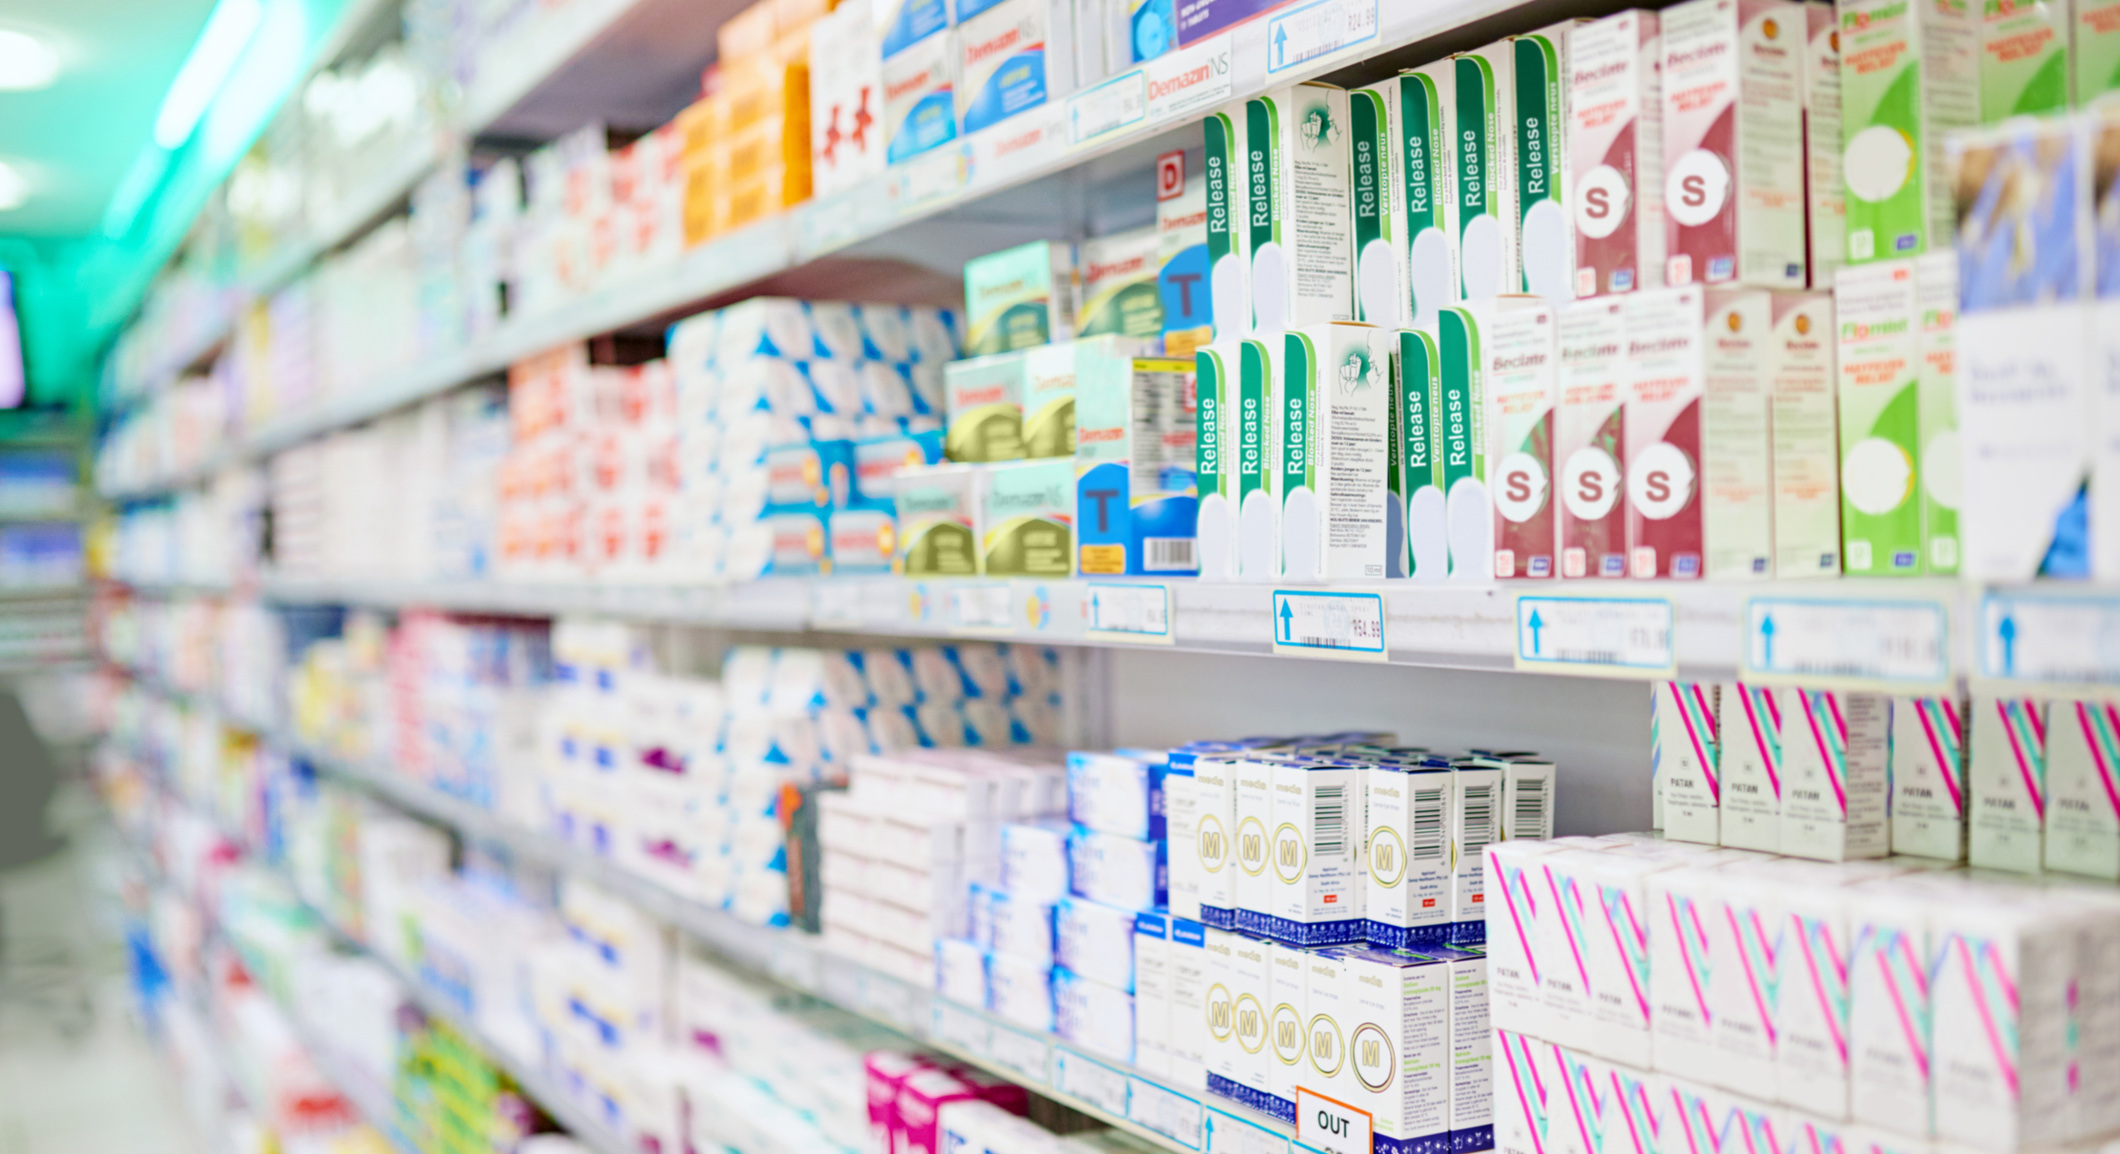
\includegraphics[width=300]{med.jpg}
\caption{Médicament}
\end{center}

\end{figure}


\subsection{Le développement du médicament}
 il y a plusieurs étape telle que :
\begin{enumerate}
\item Produire la molécule sélectionnée (principe actif) en quantité satisfaisante.
\item Tester le candidat-médicament, pour évaluer ses effets d'efficacité et ses effets indésirables (études précliniques). 
\item Rendre la molécule administrable sous une forme adaptée (comprimé, solution pour injection, patch, sirop, crème…).
\item Tester (si les étapes précliniques sont satisfaisantes), le médicament chez l'homme, dans le cadre d'essais cliniques \cite{ref7}.
\end{enumerate}
\subsection{Dénomination des médicaments}
On distingue plusieurs noms pour un médicament :
\begin{enumerate}
\item Le nom chimique qui correspond à la formule chimique exemple : acide acetyl salicylique
\item la dénomination commune international :aspirine
\item Les noms commerciaux :Aspegic ,Kardegic ,etc.
\end{enumerate}
\newpage
\section{Les molécules}
\subsection{Définition}
\textbf{Une molécule} est une structure de base de la matière. L'Union internationale de chimie pure et appliquée définit la molécule comme une entité électriquement neutre comprenant plus d'un atome,  C'est l'assemblage chimique électriquement neutre d'au moins deux atomes, différents ou non, qui peut exister à l'état libre \cite{ref8} .\\
\begin{figure}[h]
\begin{center}
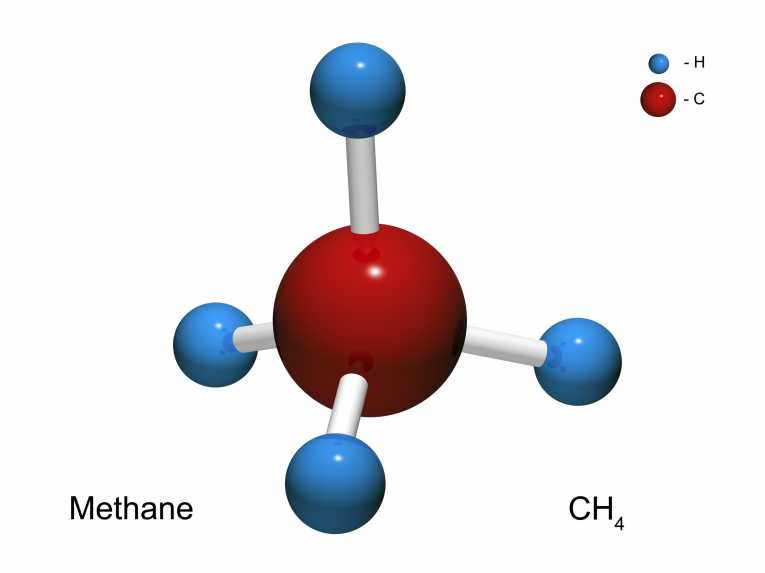
\includegraphics[width=300]{mol.jpg}
\caption{Molécule de methane}
\end{center}
\end{figure}

\subsection{Types particuliers de molécules}
\begin{enumerate}
\item L'étude des composés biochimiques a conduit les chimistes à distinguer les molécules organiques et inorganiques. 

\item Une molécule élémentaire ou \textbf{homonucléaire } est une molécule constituée d'un seul type d'atomes, par exemple le dioxygène (O2). 

\item Une molécule polaire ou \textbf{apolaire} est respectivement une molécule ayant un moment dipolaire résultant non nul (cas de la molécule d'eau) ou nul.

\item Molécule médicamenteuse : on appelle abusivement molécule la substance active d'un médicament (par opposition à son nom de marque).

\item Une molécule \textbf{amphiphile} est une molécule ayant une ou plusieurs parties hydrophiles et une ou plusieurs parties hydrophobes.

\end{enumerate}

\subsection{Le niveau moléculaire}
La structure des organismes biologiques qui constituent la biosphère peut être décomposée en plusieurs niveaux d'organisation : atomique, moléculaire, cellulaire, tissulaire, organique, des systèmes nerveux, et enfin celui de l'organisme dans sa totalité fonctionnelle. L'étude du niveau des molécules permet de comprendre le fonctionnement de la cellule, qui est l'unité fonctionnelle élémentaire du vivant \cite{ref8} .

\subsection{Molécule dans le milieu médicament}
On utilise souvent le terme de molécule pour parler du principe actif d'un médicament, Il ne faut pas confondre l'idée ancienne de principe actif, associée à celle de sa purification réalisée à partir de substances naturelles, avec celle moderne de molécule. S'il existe encore des médicaments qui contiennent des principes actifs extraits de plantes, notamment la plupart des produits pharmaceutiques modernes contiennent des substances actives dont on connaît bien la structure chimique de leur molécule \cite{ref8}. 
\newpage
\section{QSAR}
\subsection{introduction}
Le point de départ consiste à identifier une méthode efficace pour trouver un candidat-médicament actif sur une cible biologique. plus lorsque les propriétés ou structures physiochimiques sont exprimées par des chiffres, on peut proposer une relation mathématique, ou relation quantitative structure à activité, entre les deux. L'expression mathématique obtenue peut alors être utilisée comme moyen prédictif de la réponse biologique pour des structures similaires \cite{ref9} .

\subsection{Définition}
les molécules similaires ont une activité similaire. Le principe des méthodes \textbf{Qsar} consiste à mettre en place une relation mathématique à l'aide de méthodes d'analyse des données, relient des propriétés moléculaires microscopiques appelées descripteurs, à un effet expérimental (activité biologique, toxicité), pour une série des composé chimiques similaires \cite{ref9}.\\
Qsar la plus commune est de la forme : activité = f(propriétés physico-chimiques et/ou structurales).\\
\begin{figure}[h]
\begin{center}

\includegraphics[width=300]{qsar22.png}
\caption{Stilbene}
\end{center}
\end{figure}

\subsection{Domaine d'application}
L'utilisation de modèles \textbf{QSAR} pour la gestion du risque chimique s'accroissant régulièrement et étant aussi utilisé pour des visées réglementaires (en Union européenne : enregistrement, évaluation et autorisation des produits chimiques), il est crucial d'être capable d'affirmer la pertinence des prédictions. L'espace des descripteurs chimiques engendré par un ensemble spécifique de produits chimiques est appelé domaine d'applicabilité, qui permet d'indiquer lorsqu'un composé peut être prédit \cite{ref9}.

\subsection{Descripteur}
\textbf{Les descripteurs} basés sur la composition chimique de la molécule, les topologiques, obtenus à partir de la structure bi-dimensionnelle (table de connectivité des atomes de la molécule).
\\
\begin{figure}[h]
\begin{center}
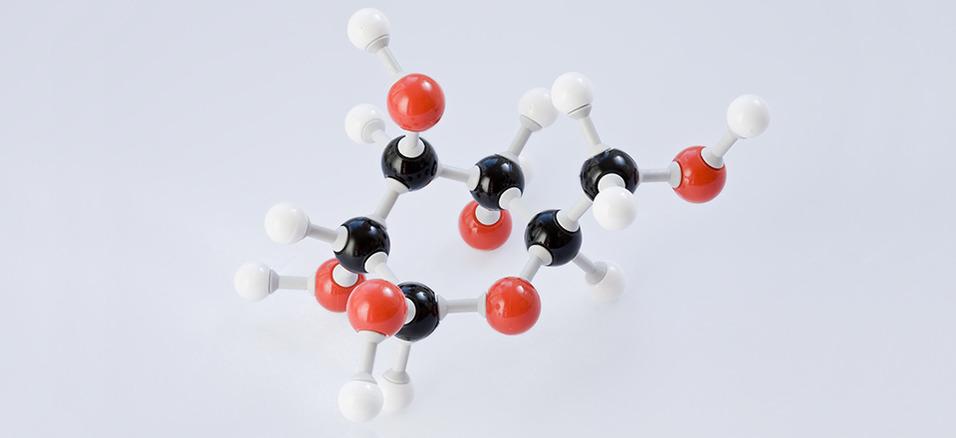
\includegraphics[width=300]{des.jpg}
\caption{Descripteur chimique}
\end{center}
\end{figure}
\subsection{Composition chimique}
La matière étant constituée en général de plusieurs corps purs (composés chimiques et corps simples), la composition chimique d'un produit fournit la quantité ou la proportion de chacun des corps purs qui le composent ; on les appelle de manière générique des composants \cite{ref9}.

\subsection{Activité biologique}
\textbf{l'activité} biologique est l'ensemble de toute les propriété moléculaire, propriété physique. l'activité biologique peut être exprimée de manière quantitative, comme pour la concentration de substance nécessaire pour obtenir une certaine réponse biologique \cite{ref9} .
\subsection{RSA et paradoxe RSA }
Le postulat de base pour les hypothèses sur des objets chimiques est que des objets similaires ont des activités similaires. Ce principe est appelé relation structure-activité (RSA, ou SAR pour structure-activity relationship en anglais). Le problème sous-jacent est donc la définition d'une petite différence sur un niveau moléculaire, chaque type d'activité, comme la réaction chimique, la biotransformation, la solubilité, l'activité de cible et d'autres encore, peuvent dépendre d'une autre différence.En général, l'intérêt est plus de trouver de fortes tendances. Les hypothèses avancées reposent habituellement sur un nombre fini de données chimiques. Ainsi, le principe d'induction devrait être respecté afin d'éviter les hypothèses surapprises et les interprétations erronées et inutiles sur les données chimiques/structurales \cite{ref9}.\\
Le paradoxe SAR est le fait que toutes les molécules similaires ne montrent pas des activités similaires. 

\subsection{Qsar en chimie}
Une des premières applications de la Qsar concernait la prédiction des points d'ébullition.Il est bien connu par exemple que pour une famille de composés chimiques, particulièrement en chimie organique, il existe une corrélation forte entre la structure et les propriétés observées \cite{ref9}.

\subsection{Qsar en biologie}
L'activité biologique des molécules est mesurée habituellement au moyen d'essais afin d'établir le niveau d'inhibition d'une transduction de signal ou d'une voie métabolique particulière. Les produits chimiques peuvent être biologiquement actifs par leur toxicité. La recherche de médicament implique parfois l'utilisation de la Qsar afin d'identifier les structures chimiques pouvant présenter de bons effets inhibiteurs sur des cibles spécifiques et possèdent une faible toxicité.

\section{Conclusion}
Tout a long de ce chapitre, nous avons pu nous rendre compte de l'avancée impressionnante de la science moderne dans le domaine de la biochimie. L'évolution de la biochimie a une influence non négligeable sur la société humaine. Elle pourrait la transformer radicalement, pour le meilleur ou pour le pire. Face aux nombreux bénéfices qui en résulteraient, les valeurs morales nous empêchent d'aller trop vite.
L'intelligence artificielle (IA) a transformé durablement l'industrie des sciences biologiques, de la médecine et de la santé. Deep Learning accélérées par les GPU peuvent être utilisées pour concevoir des réseaux de neurones encore plus sophistiqués afin d'optimiser les applications de biochimie et de recherche pharmaceutique dans de nombreux domaines .
Dans le prochain chapitre, nous allons présenter quelque concepts et définitions sur  le deep learning et les différentes utilisations dans la vie biochimie.


\end{document}

\newpage
 .
\documentclass[12pt]{report}
\usepackage{graphicx}
\usepackage{color}

\begin{document}

\chapter{Deep learning}
\begin{center}
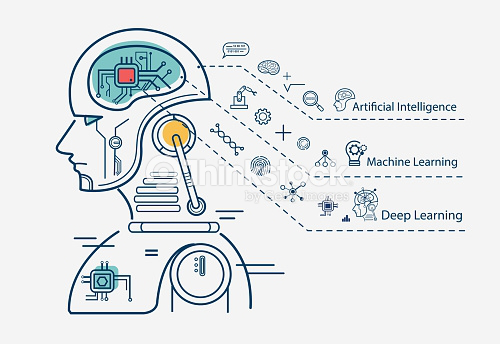
\includegraphics[width=300]{1.png} 
\end{center}

\newpage
\section{Introduction}
Au cours des dernières années, l'intelligence artificielle (IA) a fait l'objet d'un battage médiatique intense. L'apprentissage automatique, l'apprentissage en profondeur et l'IA apparaissent dans d'innombrables articles, souvent en dehors des publications axées sur la technologie .Alors abordons ces questions: qu'a-t-on appris jusqu'à présent l'apprentissage profondeur? Quelle est son importance? Où nous allons ensuite?
\\
  l'apprentissage en profondeur est un progrès relativement récent dans la programmation de réseaux de neuronaux, l'apprentissage en profondeur est composé d'un certain nombre de technologies différentes \cite{ref10} .\\
  Ce chapitre vous donnera une compréhension fondamentale de ce qu'est l'apprentissage en profondeur, de ce qu'il peut accomplir et de son fonctionnement, Cela vous familiarisera également avec le processus canonique de résolution de problèmes de données utilisant un apprentissage approfondi \cite{ref10} . 
    \\
  ce chapitre comporte la notion d'apprentissage automatique et ça puissance avec les méthodes et les technique utilisé par l'apprentissage profondeur      
 et les différentes algorithmes aussi les types de modelés de prédiction tel que la régression  et classification \cite{ref10} .

\newpage
\section{L'apprentissage automatique}

\subsection{Introduction}

L'apprentissage automatique est un sous-domaine de l'intelligence artificielle(IA). En général, l'objectif de l'apprentissage automatique est de comprendre la structure des données et de les intégrés dans des modèles qui peuvent être compris et utilisés par tout le monde \cite{ref10}.
 Les algorithmes d'apprentissage automatique permettant aux ordinateurs de s'entraîner sur les entrées de données et utilisent l'analyse statistique pour produire des valeurs qui se situent dans une plage spécifique. Pour cette raison, l'apprentissage automatique facilite l'utilisation des ordinateurs dans la construction de modèles à partir de données d'échantillonnage afin d'automatiser les processus de prise de décision en fonction des données saisies.

\subsection{Définition}
l'apprentissage automatique en anglais machine learning,ou l'apprentissage statique est un champ d'étude de l'intelligence artificielle qui se fonde sur des approches statistiques pour donner aux ordinateurs la capacité d'apprendre à partir de données, c'est-à-dire d'améliorer leurs performances à résoudre des tâches sans être explicitement programmés pour chacune.\\ Plus largement, cela concerne la conception, l'analyse, le développement et l'implémentation de telles méthodes \cite{ref11} .

\subsection{Différentes méthodes d'apprentissage automatique}
  \subsubsection{Apprentissage supervisé}
utilisé certaines variable pour prédire des valeurs inconnues au future d'autres variables par rapport la variable cible se base en deux modèle la régression et la classification. Dans la section suivante, nous allons nous intéresser plus particulièrement à la régression \cite{ref11} .



\subsubsection{Apprentissage non supervisé}
Trouver des formes interprétables par un humain permettant de décrire les données sans utiliser de variables cible à prédire \cite{...} .
\\
 le clustering est parmi l'apprentissage non supervisé qui basent sur une mesure de similarité, est généralement mesurée en termes de distances \cite{ref11} .


\subsubsection{Apprentissage semi supervisé}
Effectué de manière probabiliste ou non, il vise à faire apparaitre la distribution sous-jacente dans leur espace de description. Il est mis en œuvre quand des données manquent,Le modèle doit utiliser des exemples non étiquetés pouvant néanmoins renseigner \cite{ref11} .
\subsubsection{Différence entre l'apprentissage supervisé et non supervisé }
l'apprentissage non supervisé + label = l'apprentissage supervisé.\\

\begin{figure}[h]
\begin{center}
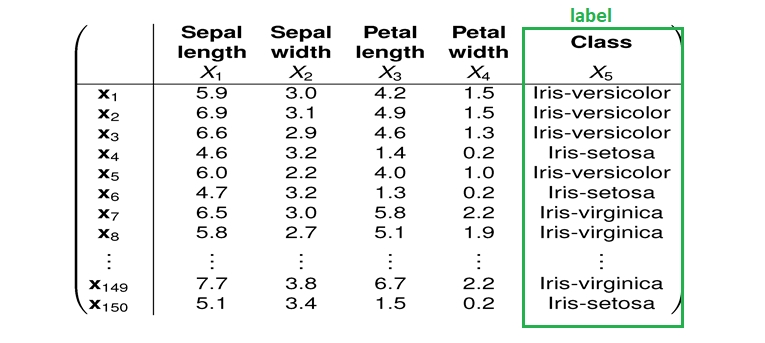
\includegraphics[width=300]{iris.jpg} 
\caption{Data Iris}
\label{Data Iris}
\end{center}

\end{figure}

aussi l'apprentissage supervisé basé sur la notion de train Data on prend par exemple sur l'ensemble des données Iris data \cite{ref11} .


\subsubsection{Prédiction}
La prédiction consiste à estimer la valeur d'une variable continue dit cible ou dépendante.  La variable cible peut représenter :
\begin{enumerate}
\item la classe à laquelle appartient chaque point de données ou
\item Un attribut mesurable 
\end{enumerate}

\subsection{Modèle prédictif et modèle descriptif}
Un modèle prédictif suppose la présence d'une variable cible alors qu'un modèle descriptif n'en suppose aucune.\\
Dans un modèle prédictif, l'analyse est guidée par la variable cible \cite{ref11}. 

\section{prédiction du variable cible}
Deux façons de faire selon le type de la variable cible :
\begin{enumerate}
\item \textbf{Régression}
\item \textbf{Classification} 

\end{enumerate}

\subsection{Modèle de régression}

\subsubsection{Définition}
Une méthode statistique qui permet d'étudier le type de relation pouvant exister entre une certaine variable (dépendante) dont on veut expliquer les valeurs et une ou plusieurs autres variables explicatives qui servent à cette explication (variables indépendantes) \cite{ref11} . \\
Le modèle de régression est un modèle prédictif qui permet d'expliquer une variable cible quantitative par une ou plusieurs variables explicatives quantitatives.





\begin{enumerate}
\item Régression linéaire simple

\item Régression linéaire multiple

\item Régression non linéaire
\end{enumerate}


\subsubsection{Régression linéaire simple}
dite simple si elle permet de prédire les valeurs d’une variable cible (expliquée (Y)) à partir des valeurs prises par une autre variable dite (explicative (X)) \cite{ref11} . \\
Ainsi, une régression linéaire simple va permettre de résumer, d’interpréter et de prévoir les variations d’une variable dépendante (Y) en fonction d’une autre variable dite indépendante (X) et ce en utilisant une droite.

\subsubsection{Régression linéaire multiple}
dite multiple si elle permet de prédire les valeurs d’une variable cible(expliquée (Y)) à partir des valeurs prises par plusieurs autres variables dites indépendantes (explicatives (Xi)) \cite{ref11}.
\subsubsection{Régression non linéaire}
La régression non linéaire est une méthode permettant de déterminer un modèle non linéaire de relation entre la variable la variable cible et un groupe de variables indépendantes (explicatives (Xi)).a l'inverse de la régression linéaire classique, qui se limite aux modèles linéaires de prévision, la régression non linéaire peut élaborer des modèles avec des relations arbitraires entre variables dépendantes et indépendantes.
\begin{figure}[h]
\begin{center}
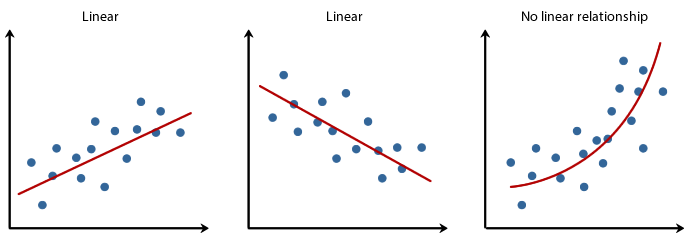
\includegraphics[width=300]{rg.png}
\end{center}
\caption{}
\label{}
\end{figure}




\subsection{Modèle de classification}
\subsubsection{Définition}
La classification supervisée permet de prédire si un élément est membre d’un groupe ou d’une catégorie donnée. 

\subsection{Classement et Classification }
Le \textbf{Classement} consiste à placer chaque individu dans une classe, parmi plusieurs classes prédéfinies en fonction des caractéristiques.\\\\
La \textbf{classification} consiste à regrouper les individus d'une population en un nombre limité de classes qui ne sont pas prédéfinies mais déterminées au cours de l'opération.

\subsection{Techniques de classification}

\begin{enumerate}
\item Arbres de décision
\item k-Plus Proches Voisins
\item Réseaux de neurones
\item Support Vector Machines
\end{enumerate}

\subsection{Arbre de décision}
Un modèle prédictif permettant d'obtenir par induction des conclusions plus générales à partir de faits particuliers.\\\\

\begin{figure}[h]
\begin{center}
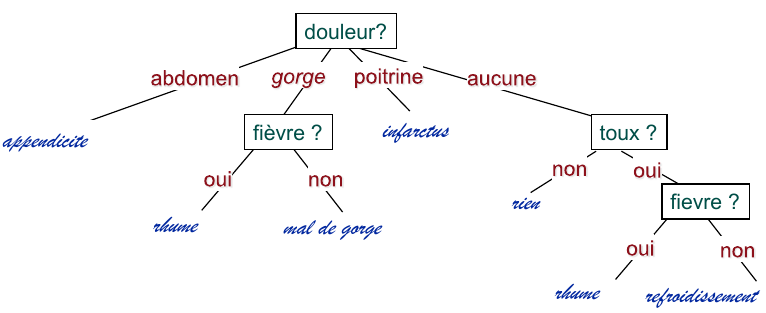
\includegraphics[width=400]{add2.png}
\caption{Arber de décision}
\label{}
\end{center}


\end{figure}

\newpage
\subsection{Structure d'un arbre de décision}
\begin{enumerate}
\item Chaque noeud interne correspond à un attribut.
\item Chaque branche correspond à valeur possible de cet attribut.
\item Chaque feuille correspond à une classe et fournit une classification.
\item Chaque chemin dans l'arbre correspond à une règle.

\end{enumerate}

\subsection{K-Plus Proches Voisins( KNN )}
C'est une méthode de classification supervisée  basée sur l'analogie.\\
C'est une des méthodes de classification les plus simples.\\\\

\begin{figure}[h]
\begin{center}
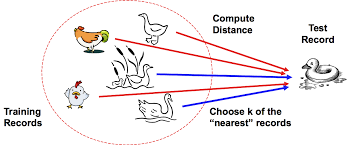
\includegraphics[width=400]{knn.png}
\caption{K-plus proches voisin}
\label{K-plus proches voisin}
\end{center}
\end{figure}
\\\\
Choix de la distance par attribut et du mode de combinaison des distances.






%la partie 2eme consernent le Deep learning trée important

\newpage
\section{Deep learning}

\subsection{Définition}
 est un ensemble des méthodes d’apprentissage automatique tentant de modéliser avec un haut niveau d’abstraction des données grâce à des architectures articulées de différentes transformations fondées sur l’apprentissage de modèles de données. Une observation (une image, p. ex.) peut être représentée de différentes façons par un vecteur de données.

\subsection{pour quoi l'utilisation de Deep learning}
Les deux idées clés de l'apprentissage en profondeur pour la vision par ordinateur - réseaux de neurones convolutionnels et rétropropagation - étaient déjà bien comprises en 1989. L'algorithme LSTM (Long Short Term Memory), fondamental pour un apprentissage en profondeur pour la série temporelle, a été développé en 1997.
 et a à peine changé depuis. Alors pourquoi l'apprentissage en profondeur n'a-t-il démarré qu'après 2012? Qu'est-ce qui a changé dans ces deux décennies?
En général, trois forces techniques sont à l'origine des progrès de l'apprentissage automatique:
\begin{enumerate}
\item  matériel
\item  Jeux de données
\item l'avancement d'algorithmiques
\end{enumerate}
\\
Les algorithme de machine learning n’est pas efficace pour les données volumineuses,Le deep learning est capable de traiter les données volumineuses.\\
dans le deep learning, on utilise un réseau de neurones artificiels qui a pour but d'apprendre seul à résoudre le problème, à l'aide d'une ensemble de données.

\subsection{La démocratisation de l'apprentissage profondeur}
La démocratisation des outils utilisés sur le terrain est l’un des facteurs clés de cet afflux de nouveaux visages dans l'apprentissage en profondeur \cite{ref12} . À ses débuts, l'apprentissage en profondeur nécessitait une expertise considérable en C ++ et CUDA, que peu de gens possédaient. De nos jours, les compétences de base en scripts Python suffisent pour effectuer des recherches approfondies en profondeur. Cela s’explique notamment par le développement de Theano, puis de TensorFlow, deux frameworks symboliques de manipulation tenseur pour Python prenant en charge l'autodifférenciation, simplifiant grandement la mise en œuvre de nouveaux modèles, et par la montée en puissance de bibliothèques conviviales telles que Keras, ce qui rend l'apprentissage en profondeur aussi facile que la manipulation de briques LEGO. Après sa sortie au début de 2015, Keras est rapidement devenu la solution d'apprentissage en profondeur par excellence pour un grand nombre de nouvelles entreprises en démarrage, d'étudiants diplômés et de chercheurs sur le terrain.

\subsection{Les réseaux de neurones artificiel (ANNs)}
Un réseau de neurone artificiel, ou réseau neuronal artificiel, est un système dont la conception est à l'origine schématiquement inspirée du fonctionnement des neurones biologiques, et qui par la suite s'est rapproché des méthodes statistiques \cite{ref12} .\\
\begin{figure}[h]
\begin{center}
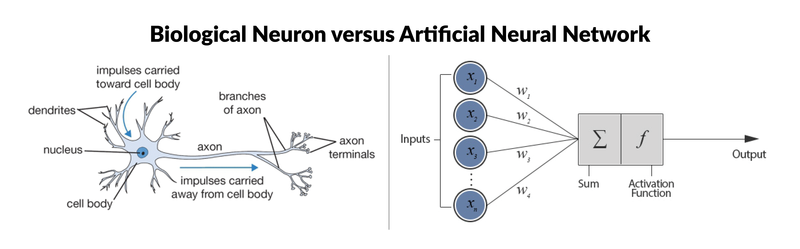
\includegraphics[width=450]{bio.png}
\caption{réseau neuronal}

\end{center}
\end{figure}


utiliser pour extraire des règles et des tendances à partir de données compliquées, bruitées et imprécises. Ils peuvent s'utiliser pour extraire des modèles et détecter des tendances reposant sur des fonctions mathématiques compliquées qui sont trop difficiles, voire impossible, à modéliser à l'aide de techniques analytiques ou paramétriques traditionnelles \cite{ref12} .
\subsection{Les taches des réseaux de neurones (ANNs) }
les réseaux de neurones sont en mesure d'effectuer différentes catégories de tâches, notamment de la \textbf{régression} et de la \textbf{classification}, Les tâches de régression visent à mettre en relation un certain nombre de variables d'entrée x avec un ensemble de résultats continus t (les variables cible). Par opposition, les tâches de classification visent à affecter des observations aux classes d'une variable cible catégorielle en fonction d'un ensemble de valeurs d'entrée \cite{ref13} .

\subsection{Utilisation des Réseaux de Neurones}
Les réseaux de neurones ont une remarquable faculté à donner un sens, extraire des règles et des tendances à partir de données compliquées, bruitées et imprécises. Ils peuvent s'utiliser pour extraire des modèles et détecter des tendances reposant sur des fonctions mathématiques compliquées qui sont trop difficiles, voire impossible, à modéliser à l'aide de techniques analytiques ou paramétriques traditionnelles \cite{ref13} .  les réseaux de neurones sont particulièrement bien adaptés à l'application de problématiques concrètes dans les domaines de la recherche scientifique, un certain nombre de domaines dans lesquels les réseaux de neurones ont été appliqués avec succès :

\begin{enumerate}
\item Robotique
\item Classification
\item Analyse de l'image et synthèse vocale
\item Diagnostiques et suivi médical

\end{enumerate}
 



\subsection{Les réseaux de neurones convolutif (CNN)}
Le réseau de neurones convolution (CNN) est une technologie de réseau de neurones qui a eu un impact profond sur le domaine de la vision par ordinateur (VC).Fukushima en 1980 a introduit le concept original d'un réseau de neurones convolutionnel. \\
la convolution est une technologie importante souvent combiné avec l'apprentissage profondeur \cite{ref13} . Hinton en 2014 a introduit la convolution pour permettre aux réseaux de reconnaissance d'images de fonctionner de la même manière que les systèmes biologiques et d'obtenir des résultats plus précis \cite{ref13} .\\
\newpage
\subsection{Définition}
réseaux d'unités de calcul élémentaire inter connectées,algorithmes pour résoudre des problèmes complexes.Le réseau de neurones artificiels est un moyen de modélisation du mécanisme d'apprentissage et de traitement de l'information qui se produit dans le cerveau humain afin de reproduire certaines caractéristiques \cite{ref13}   .\\
Déterminer un réseau de neurones = Trouver les coefficients synaptiques.\\
On parle de phase d'apprentissage : les caractéristiques du réseau sont modifiées jusqu'à ce que le comportement désiré soit obtenu.

\subsection{Structure de base de CNN}
Une conception typique de CNN commence par l'extraction des caractéristiques et se termine par la classification. L'extraction des caractéristiques est effectuée en alternant des couches de convolution avec des couches de sous-échantillonnage. La classification est effectuée avec des couches denses suivies d'une couche finale softmax. Pour la classification des images, cette architecture fonctionne mieux qu'un réseau de neurones à rétroaction intégrale entièrement connecté \cite{ref13} .
\begin{figure}[h]
\begin{center}
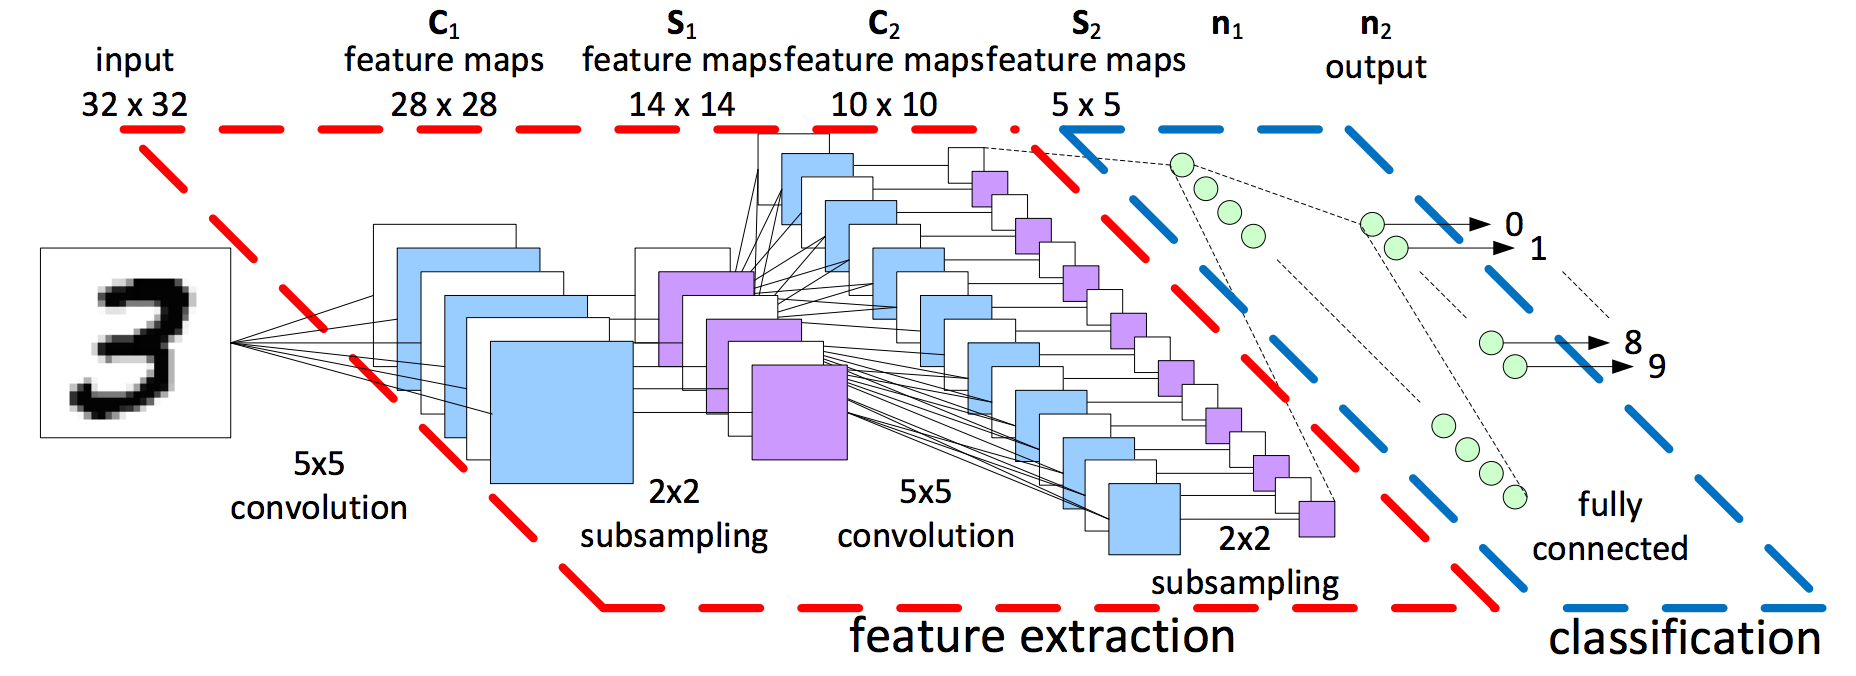
\includegraphics[width=300]{extract.png}
\caption{Structure de CNN}
\label{Structure de CNN}
\end{center}
\end{figure}


\subsection{Les Couches utilisées pour construire des CNN}
Comme nous l'avons décrit ci-dessus, un ConvNet simple est une séquence de couches et chaque couche d'un ConvNet transforme un volume d'activations en un autre à l'aide d'une fonction différentiable. Nous utilisons trois types principaux de couches pour construire des architectures ConvNet: la couche convolutionnelle, la couche de regroupement et la couche entièrement connectée (exactement comme dans les réseaux de neurones normaux). Nous allons empiler ces couches pour former une architecture ConvNet complète \cite{ref14}.
\begin{figure}[h]
\begin{center}
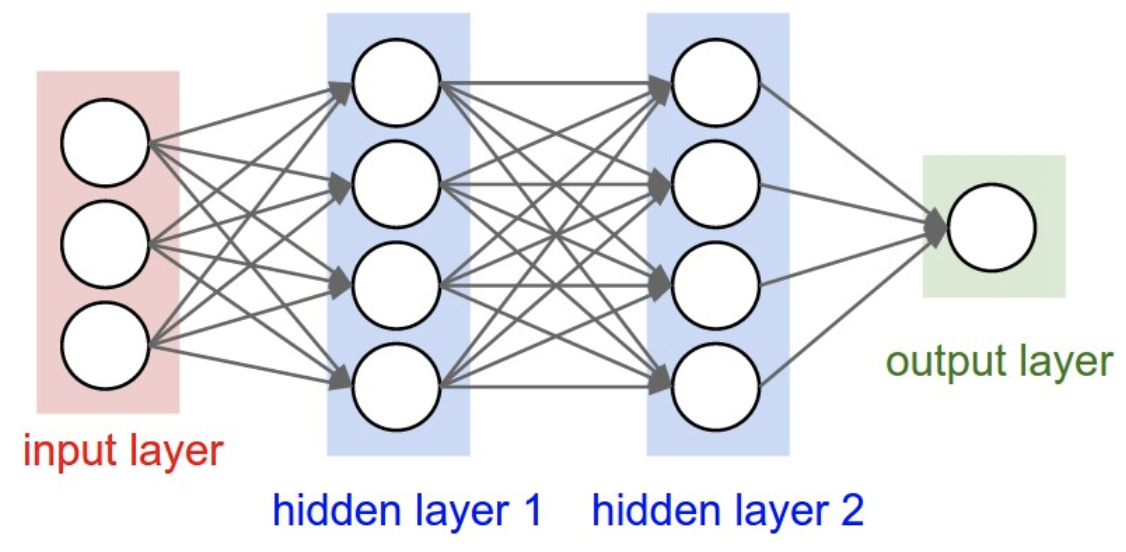
\includegraphics[width=300]{nnda.png}
\caption{Les couches de CNN}
\label{Les couches de CNN}
\end{center}
\end{figure}



\subsection{Caractéristiques et avantages CNN}
Un avantage majeur des réseaux convolutifs est l'utilisation d'un poids unique associé aux signaux entrant dans tous les neurones d'un même noyau de convolution.Cette méthode réduit l'empreinte mémoire, améliore les performances et permet une invariance du traitement par translation \cite{ref14}.\\
C'est le principal avantage du réseau de neurones convolutifs par rapport au perceptron multicouche, qui lui considère chaque neurone indépendant et affecte donc un poids différent à chaque signal entrant.

\subsection{Architecture de CNN}
Plusieurs architectures dans le domaine des réseaux de convolution Les plus courants sont:
\subsubsection{LeNet}
Les premières applications réussies de réseaux de convolution ont été développées par Yann LeCun dans les années 1990. Parmi celles-ci, la plus connue est l'architecture LeNet utilisée pour lire les codes postaux, les chiffres, etc \cite{ref15} .
\subsubsection{AlexNet}
Le premier travail qui a popularisé les réseaux de convolution dans la vision par ordinateur a été AlexNet, développé par Alex Krizhevsky, Ilya Sutskever et Geoff Hinton  .
\subsubsection{GoogLeNet}
ILSVRC 2014 était un réseau de convolution de de Google, Sa principale contribution a été la mise au point d'un module de démarrage réduisant considérablement le nombre de paramètres dans le réseau (4 M, par rapport à AlexNet avec 60 M) \cite{ref15}.



\subsection{LeNET-5}
LeNET-5 est une architecture primaire du classification pour l'images graphiques, le réseau LeNET-5 contient plusieurs types de couche diffirent et données flux de l'entrée à la sortie.
\begin{figure}[h]
\begin{center}
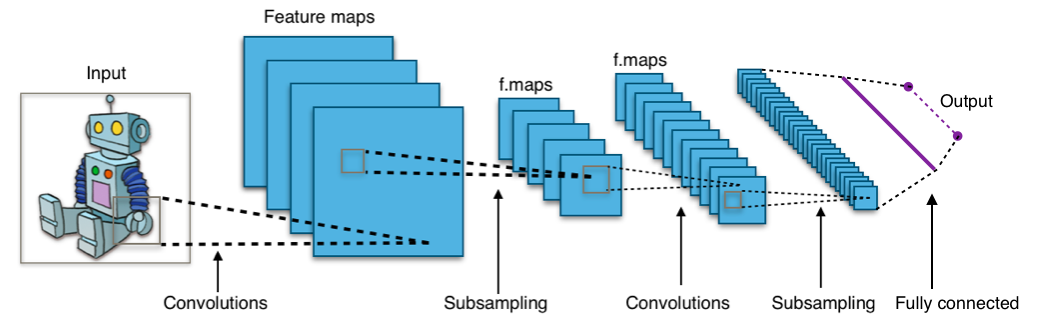
\includegraphics[width=400]{cnn.png}
\caption{LeNET-5}

\end{center}
\end{figure}
\\
Dans le cadre de la reconnaissance d'image, cette dernière est ( pavée ), c'est-à-dire découpée en petites zones (appelées tuiles). Chaque tuile sera traitée individuellement par un neurone artificiel (qui effectue une opération de filtrage classique en associant un poids à chaque pixel de la tuile) \cite{ref15}.



\newpage
\subsection{Ensembles d'apprentissage et d'évaluation}
Un\textbf{ ensemble d'évaluation }est un ensemble de données utilisé pour évaluer le modèle développé à partir d'un ensemble d'apprentissage \cite{ref15} .% par google
\\
par exemple,nous avons obtenu énormément de données nous pouvont diviser l'ensemble de données en deux partie,avec un ensemble  sera grand que l'autre puis en utiliser la partie grande pour l'apprentissage et l'autre pour l'évaluation \cite{ref15} .

\subsection{Données de qualité}
Évidemment, si vos données d'entraînement sont pleines d'erreurs, de valeurs aberrantes et de bruits (en raison de mesures de mauvaise qualité, par exemple), il sera plus difficile pour le système de détecter les modèles sous-jacents. Par conséquent, votre système sera moins performant. Cela vaut souvent la peine de passer du temps à nettoyer vos données de formation. En réalité, la plupart des scientifiques de données consacrent une grande partie de leur temps à cela  \cite{ref16}.

\subsection{Entraînement et Validation}
La création d'un ensemble d'apprentissage et d'un ensemble d'évaluation à partir d'un ensemble de données vous permet de déterminer si un modèle spécifique généralisera bien les nouvelles données \cite{ref15} .\\
\begin{figure}[h]
\begin{center}
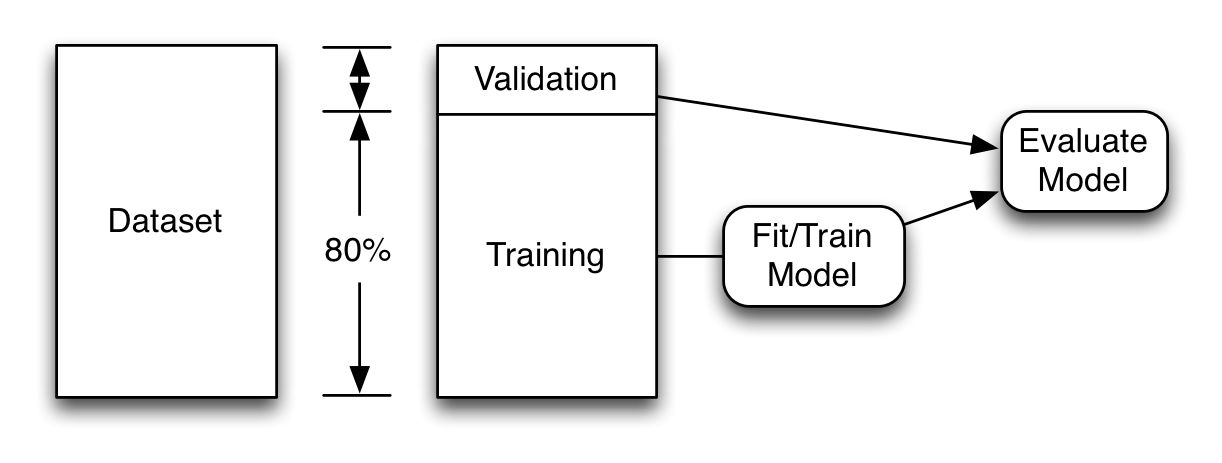
\includegraphics[width=300]{evalu.png}
\caption{Entrainement et Validation}

\end{center}

\end{figure}


 Il existe deux moyens principaux de traiter les données de formation et de validation:
\subsubsection{Entraînement/validation split}
Les données sont réparties selon un certain rapport entre un ensemble de évaluation et de validation. Les ratios habituels sont \textbf{80/100}  pour entrainement formation et \textbf{20/100}  pour validation  \cite{ref16}.

\subsubsection{K-Fold Cross Validation}
Les données sont divisées en un certain nombre de plis et de modèles. Étant donné qu'un nombre de modèles égal aux plis est créé, des prédictions hors échantillon peuvent être générées pour l'ensemble du jeu de données  \cite{ref17}.

\subsection{Représentation}
Un modèle de Machine Learning ne peut pas directement voir, entendre ou sentir les exemples d'entrée. Vous devez donc créer
une\textbf{ représentation }des données pour fournir au modèle un angle de vue utile sur les qualités clés des données. Autrement dit, pour entraîner un modèle, vous devez choisir l'ensemble de caractéristiques qui représentent le mieux les données.\\
Certaines représentations et une bonne capacité d’analyse automatique des différenciations rendent la tache d'apprentissage plus efficace.




\newpage
\section{Conclusion}
Les systèmes d'apprentissage en profondeur représente ensemble des tache qui amélioré la précision avec des outils très puissant qui permet d'effectuer de multiples actions encore de créer un programme évolutionnaire qui s'améliore sans cesse. Le présent document est centré sur la manière dont l'apprentissage en ensemble peut être appliqué à ces différents systèmes d'apprentissage en profondeur pour obtenir une plus grande précision de reconnaissance \cite{ref17}.\\
les réseaux de neurones convolutionnels est un domaine très actif dans le domaine de la vision par ordinateur.

\newpage
\bibliographystyle{plain}
\bibliography{biblioDeep}

\end{document}




\newpage
.
\documentclass[12pt]{report}
\usepackage{graphicx}
\usepackage{color}

\begin{document}


\chapter{La Bioinformatique}

\begin{center}
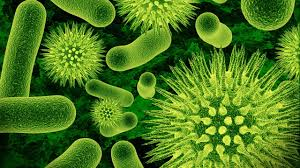
\includegraphics[width=300]{bio.jpg} 
\end{center}






\newpage
\section{Intoduction}
La bioinformatique est une "interdiscipline" à la frontière de la biologie, de l'informatique et des mathématiques. Les systèmes biologiques sont très complexes et les techniques modernes d'investigation du monde biologique fournissent une vaste quantité de données expérimentales. Le but ultime de la bioinformatique est d'intégrer ces données d'origines très diverses pour modéliser les systèmes vivants afin de comprendre
et prédire leurs comportements (biologie systémique ou biologie des systèmes) dans des conditions de fonctionnement normales ou pathologiques. La bioinformatique est donc étroitement couplée à ses applications. Bon nombre de bioinformaticiens ne travaillent pas dans des laboratoires formellement estampillés \cite{ref18} . 
\\
Aujourd'hui , tout projet de biologie comporte une étape d'analyse bioinformatique des données. Par conséquent, un biologiste passe environ 20-30/100 de son temps à utiliser des outils bioinformatiques.\\
Ce chapitre décrit de manière simple les tâches courantes de la bioinformatique qu'un biologiste/biochimiste doit savoir traiter par lui-même, a partir les progrès de l'intelligence informatique pour la bioinformatique qui nous avons utiliser pour notre contexte d'étude qui représente l'application de l'apprentissage profond pour la prédiction de l'activité biologie \cite{ref18} .
\newpage
\section{Histoire du terme bioinformatique}
Le terme de bioinformatique date du début des années 80. Cependant, le concept sous-jacent de traitement de l'information biologique est bien plus vieux. Durant les années 60, la biologie moléculaire a eu besoin de modélisation formelle, ce qui a mené à la création des bioinformatique \cite{ref19}.\\
\section{Pour quoi la bioinformatique}
La bioinformatique est l'étude de l'information biologique. Ce n'est pas simplement l'application à la biologie de l'informatique, c'est une branche à part entière de la biologie. La bioinformatique actuelle se concentre surtout sur l'étude des séquences d'ADN et sur le repliement des protéines, donc travaille surtout au niveau moléculaire \cite{ref19} . 
\section{Qu'est-ce que la bioinformatique }
\subsection{Définition}
La bioinformatique est l'étude de l'information biologique de façon automatique, alors elle inclut la création et le développement de technologies informatiques qui permettant le traitement et l'analyse de ces information.
\\
l'intégration des méthodes mathématiques ,statistiques ,informatiques  pour analysées des données biologiques ,biochimiques et biophysiques \cite{ref20} .

\begin{figure}[h]

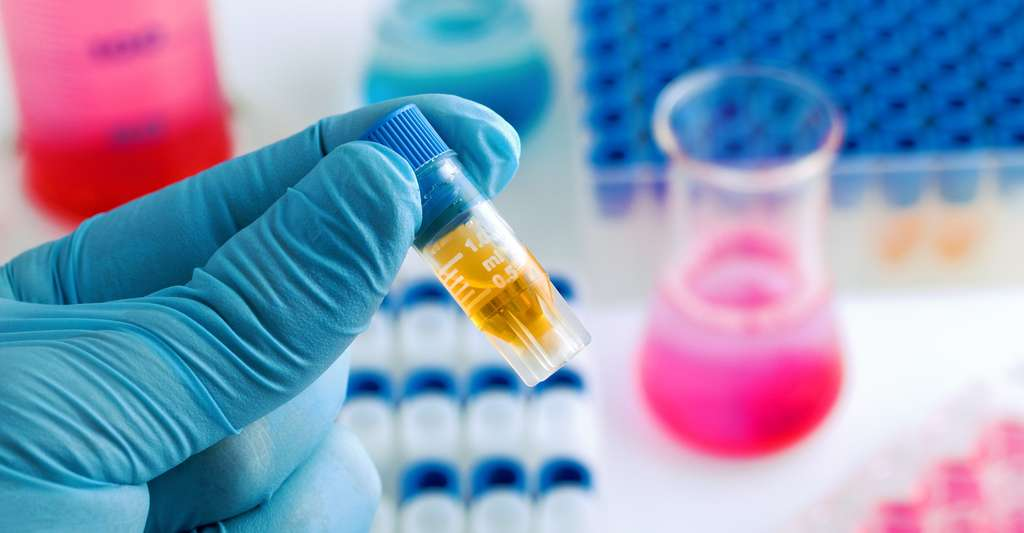
\includegraphics[width=200]{bb.jpg} 
\caption{premier image}
\label{premier image}

\end{figure}


La bioinformatique  se réfère spécifiquement à la recherche et à l'utilisation de  patterns et structures dans les données biologiques et au développement de nouvelles méthodes pour accéder aux bases de données \cite{ref20} .
\section{Apports à la biologie}
L'informatique est devenue un apport fondamentale à la biologie moléculaire. Les moyens informatiques sont naturellement utilisés pour le stockage ou la gestion des données mais également pour l'interprétation de ces données. Le traitement informatique des séquences peut par exemple déterminer la fonction biologique d'un gène. Cet apport informatique concerne principalement quatre aspects :
\begin{enumerate}
\item Le premier est l'organisation des données avec essentiellement la création de bases de données afin de réunir le plus d'information possible sur les séquences. 
\item Le deuxième aspect concerne les traitements que l'on peut effectuer sur les séquences afin de repérer un élément biologique intéressant. Ces programmes représentent les traitements couramment utilisés dans l'analyse des séquences comme la recherche des similitudes d'une séquence avec l'ensemble d'une base de données.
\item Le troisième aspect est celui qui permet d'élaborer des stratégies pour apporter des connaissances biologiques supplémentaires que l'on pourra ensuite intégrer dans des traitements standards. Par exemple la mise au point de nouvelles matrices de substitution des acides aminés,...etc
\item  Enfin, le quatrième aspect est celui de l'évaluation des différentes approches citées précédemment dans le but de valider.

\end{enumerate}





\section{Domaine d'application}
De plus en plus, la bioinformatique est développée dans un but d'application à l'agriculture, la pharmacologie, la  médecine \cite{ref21}. 
\newpage
\subsection{Structures moléculaires}
  Visualisation, analyse, classification, prédiction.
  \begin{figure}[h]
  \begin{center}
  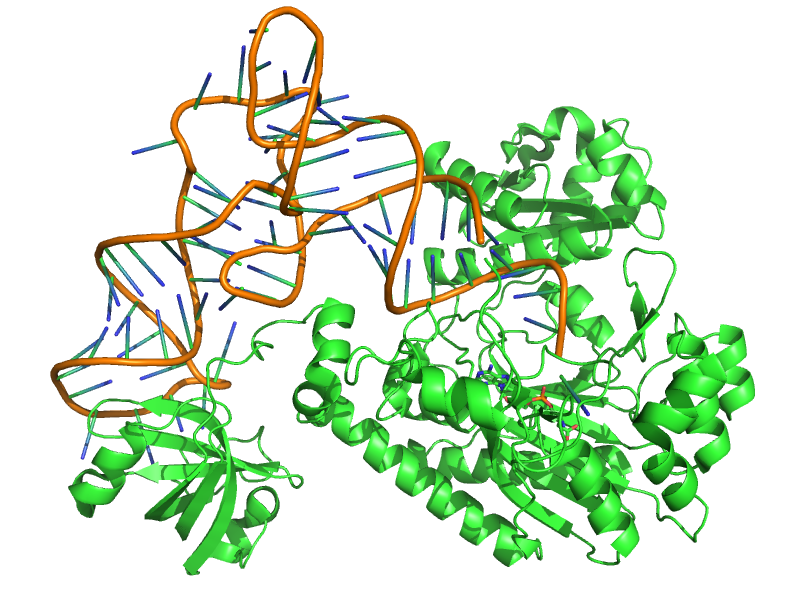
\includegraphics[width=200]{m.png} 
   \caption{La structure moléculaire}
  \end{center}  
  \end{figure}
  \subsection{Analyse de séquences}  
Alignements, recherches de similarités, détection de motifs.
\subsection{La recherche pharmaceutique}
\begin{enumerate}
\item Mécanismes d'action des médicaments.
\item Identification de cibles pharmaceutiques.
\end{enumerate}
\subsection{Génomique}
Annotation des génomes, génomique comparative.
\subsection{Analyse des réseaux biomoléculaires}
Réseaux métaboliques, d'interactions protéiques, de régulation génétique.

\newpage
\section{Quantitative et le système Pharmacologie (QSP)} 
La pharmacologie quantitative (QSP) est une nouvelle discipline sur l'identification et la validation de cibles de médicaments, comprendre les thérapeutiques existantes. Le but de QSP est de comprendre la manière précise et prédictive aussi comment les médicaments modulent les réseaux cellulaires dans l'espace et dans le temps et leur impact sur la physiopathologie humaine \cite{ref21}.\\
Au cours des trois dernières décennies, le paradigme dominant dans la découverte de médicaments a été la conception de ligands sélectifs pour une cible spécifique afin d'éviter les effets indésirables. Cependant, dans l'ère postgénomique actuelle, l'objectif est de concevoir des médicaments à partir les modèles de relations quantitatives structure-activité \textbf{QSAR} pour prédire la réponse biologique quantifiée d'une molécule à partir de ses descripteurs \cite{ref21} .

\section{Progrès de l'intelligence informatique pour la bioinformatique}
La bioinformatique est en train de devenir de plus en plus une science basée sur les données, une évolution tirée par les avancées technologiques en acquisition de données . Dans le domaine biomédical la grande quantité de données générées des scénarios difficiles pour les chercheurs, Les nouvelles exigences en matière de données requièrent de nouvelles approches en matière d'analyse des données. Certaines des plus intéressantes proviennent actuellement des domaines de l'intelligence computationnelle (IC) et de l'apprentissage automatique (ML) \cite{ref21}.\\
Cette session s'intéresse particulièrement à la proposition d'approches  de l'apprentissage automatique ML pour résoudre les problèmes dans les domaines biomédical et bioinformatique. Les sujets qui intéressent cette session :
\begin{enumerate}

\item \textbf{ Application de l'apprentissage profond pour la prédiction de l'activité biologique.}
\item Nouvelles applications des méthodes existantes d'apprentissage automatique ML à la bioinformatique.
\item Nouvelles techniques de d'apprentissage automatique ML pour la biomédecine et la bioinformatique.

\end{enumerate}
\newpage
\section{l'apprentissage profond et la modélisation Qsar}
\subsection{QSAR}
Relations entre l'industrie pharmaceutique et les modèles de relations quantitatives structure-activité (QSAR) pour prédire la réponse biologique quantifiée d'une molécule à partir de ses descripteurs, qui sont essentiellement des études étudiées de la molécule.

\begin{figure}[h]
\begin{center}
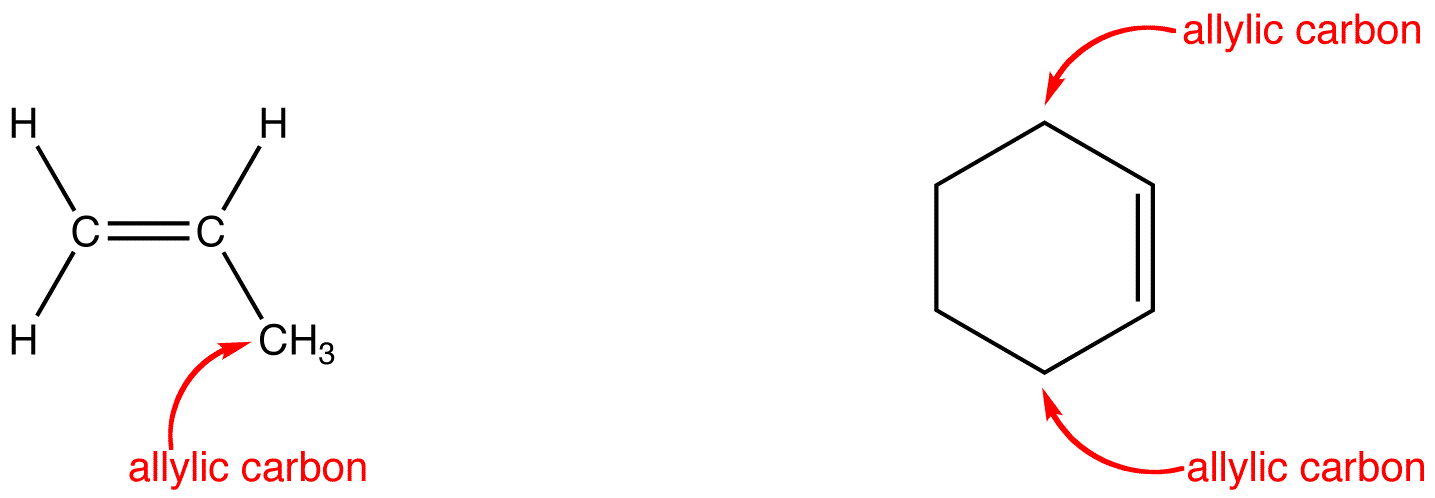
\includegraphics[width=250]{qsar.png} 
\caption{Allylic carbon}
\label{Allylic carbon}
\end{center}
\end{figure}
 
La complexité de ces descripteurs varie et peut aller de simples mesures de poids moléculaire à des caractéristiques géométriques complexes. La découverte de médicaments est un processus long et coûteux pour le secteur pharmaceutique.
\subsection{L'apprentissage en profondeur}
L'apprentissage en profondeur (deep learning) est un ensemble de méthodes d'apprentissage automatique et Les algorithmes d'apprentissage automatique, permettent aux ordinateurs de s'entrainer sur les entrées de données et utilisent l'analyse statistique .\\
fondées sur l'apprentissage de modèles de données, Une observation (une image, p. ex.) peut être représentée de différentes façons par un vecteur de données. Certaines représentations et une bonne capacité d'analyse automatique des différenciations rendent la tache d'apprentissage plus efficace \cite{ref22}.

\newpage
\subsection{La prédiction de l'activité biologique}
Le principe de la modélisation \textbf{Qsar}, consiste à trouver une relation reliant quantitativement une \textbf{activité biologique} mesurée expérimentalement. Ceci, est réalisé pour une série de composes similaire avec des descripteurs moléculaires à l'aide des méthodes computationnelles.\\
Les données des molécules biologiques disponibles dans les benchmarks sont tellement volumineuses (Big Data), qu'ils en deviennent difficiles à l'analyser avec des techniques de traitement de données classiques. Afin d'arriver à analyser ce type de données,nous faisant appel à des algorithmes de \textbf{Deep Learning }, qui sont en constante augmentation dans plusieurs domaines \cite{ref22}.

\section{Utilisation de l'amarrage (Docking)}
Dans le domaine de la modélisation moléculaire, l'amarrage est une méthode qui calcule l'orientation préférée d'une molécule vers une seconde lorsqu'elles sont liées pour former un complexe stable. Savoir l'orientation préférée sert à prévoir la solidité de l'union entre deux molécules \cite{ref23} .
\begin{figure}[h]
\begin{center}
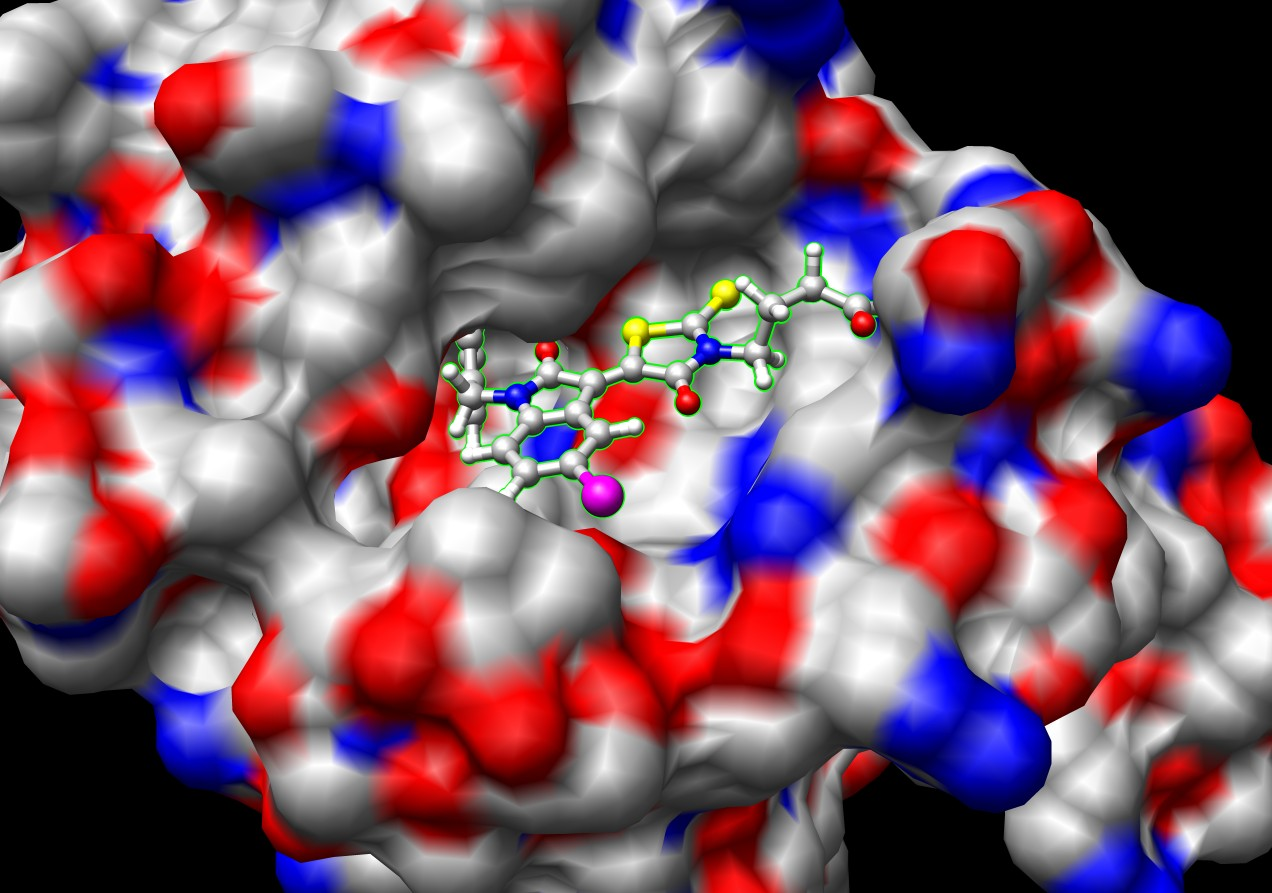
\includegraphics[width=200]{Docking.jpg}
\end{center}
\caption{Docking}
\end{figure}

 Les associations entre des molécules d'importance biologique, telles que les protéines, les acides nucléiques, les glucides et matières grasses jouent un rôle essentiel dans la transduction de signal. D'ailleurs, l'orientation relative des deux molécules associées peuvent avoir un effet sur le genre du signal produit (ex. antagoniste contre l'agoniste ). Par conséquent, des études d'amarrage sont utiles à calculer la force et le genre du signal produit  \cite{ref23} .\\
 Dans la mise au point de nouveaux médicaments, l'amarrage sert souvent à déterminer l'orientation de petites molécules liées à leurs protéines ciblées afin de calculer leurs affinité et niveau d'activité.



\section{Conclusion}
Dans ce chapitre nous avons définit les notions et l'évolution de la \textbf{bioinformatique} d'après le concept traitement de l'information biologique. les caractéristiques aussi les domaine d'application de la bioinformatique ,vers le problème biologique a traité sous domaine de la pharmacologie, d'objectif la prédiction de l'activité biologique pour concevoir des médicament à partir le modèle quantitative QSAR avec les moyennes informatique qui représente technique de l'apprentissage automatique (ML) qui fais appel à des algorithmes de Deep learning.\\
Dans le prochain chapitre nous allons exprimé notre démarche d'étude, aussi les outils de développement  utilisés tel que  le langage de programmation, sous chapitre de contribution.

\newpage
\bibliographystyle{plain}
\bibliography{biblio}

\end{document}

\newpage
.
\part{}
\chapter{Contribution}
\chapter{Résultat et discussion}
\newpage
\section*{Conclusion générale}
\newpage
\bibliographystyle{plain}
\bibliography{biblio}

\end{document}